\appendixes

\renewcommand{\appendixname}{Anexo}
\renewcommand{\appendixtocname}{Anexos}
\renewcommand{\appendixpagename}{Anexos}
%\newcounter{anexo1}
%\setcounter{anexo1}{1}
\begin{addendum}
	
	\chapter{Historias de Usuario}
	% ==========================================
	% Gestión de Usuarios y Autenticación
	% ==========================================
	
	\begin{userstory}[hu:01]
		\storyname{Registrar una nueva cuenta de usuario}
		\storyuser{Visitante del sitio web}
		\storyiter{1} % Iteración estimada
		\storypriority{Alta} % Basado en RF1
		\storyrisk{Bajo}
		\storypoints{1 semana} % Estimación basada en ejemplo
		\storyprogrammer{Daniel Rojas Grass} % Manteniendo el nombre del ejemplo
		\storydescription{
			Como visitante del sitio web, debe poder registrar una nueva cuenta proporcionando su dirección de correo electrónico, nombre de usuario y una contraseña segura, para crear una cuenta personal que la permita acceder a las funcionalidades de consulta y visualización del archivo histórico y guardar su historial de conversaciones. (Corresponde principalmente a RF1)
			
			\textbf{Precondiciones:}
			\begin{itemize}
				\item El visitante no tiene una sesión activa.
				\item El visitante se encuentra en la página o sección de registro del sitio web.
				\item El \textit{backend} está operativo y accesible.
			\end{itemize}
			
			\textbf{Flujo de acción:}
			\begin{enumerate}
				\item Visitante ingresa dirección de correo electrónico, nombre de usuario, contraseña y confirmación de contraseña en el formulario de la sección registrar cuenta.
				\item Visitante envía el formulario.
				\item El sitio web valida formato básico (e.g., dirección de correo electrónico válido, contraseñas coinciden, nombre de usuario único).
				\item El sitio web envía los datos al endpoint de registro del \textit{backend}.
				\item El \textit{backend} valida los datos (e.g., dirección de correo electrónico no existente,nombre de usuario no existente, complejidad de contraseña) y crea el usuario en la base de datos de forma segura.
				\item El \textit{backend} retorna una respuesta de éxito o error al frontend.
				\item El \textit{frontend} muestra un mensaje apropiado al usuario (éxito o error específico).
			\end{enumerate}
		}
		\storyobservation{
			Implementar validación de fortaleza de contraseña en \textit{frontend} y \textit{backend}. Asegurar almacenamiento seguro de contraseñas (hashing). Los mensajes de error deben ser claros (e.g., 'El correo electrónico ya está registrado', "Las contraseñas no coinciden").
		}
		\storyinterface{ % Inicio del contenido de storyinterface
			Formulario de registro del sitio web: % Texto descriptivo inicial
			\par\medskip % Añade un pequeño espacio vertical
			\begin{center} % Para centrar la imagen
				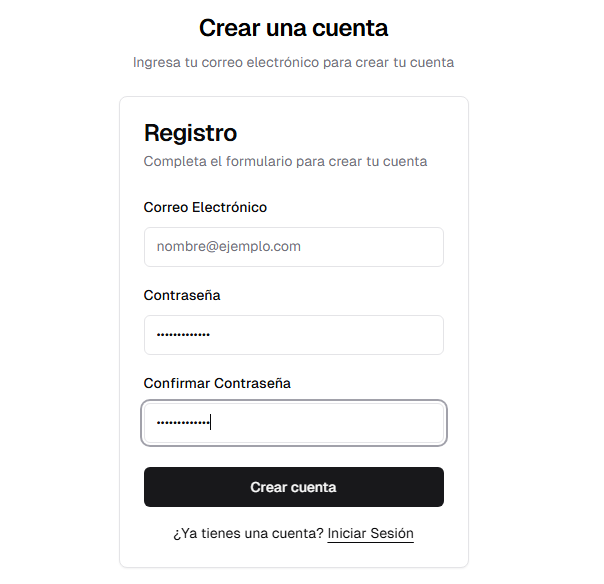
\includegraphics[width=0.6\textwidth]{images/create.PNG} % Imagen del ejemplo
			\end{center}
			\medskip % Espacio después de la imagen
		}
		
		
	\end{userstory}
	
	\begin{userstory}[hu:02]
		\storyname{Iniciar sesión en el sistema}
		\storyuser{Usuario registrado}
		\storyiter{1} % Iteración estimada
		\storypriority{Alta} % Basado en RF2
		\storyrisk{Bajo}
		\storypoints{1 semana} % Estimación basada en ejemplo
		\storyprogrammer{Daniel Rojas Grass}
		\storydescription{
			Como usuario registrado, debe poder iniciar sesión utilizando su correo electrónico y contraseña previamente registrados, mi historial de conversaciones y utilizar las capacidades completas del sistema de chat. (Corresponde principalmente a RF2, RF4)
			
			\textbf{Precondiciones:}
			\begin{itemize}
				\item El usuario tiene una cuenta previamente registrada en el sistema.
				\item El usuario no tiene una sesión activa.
				\item El usuario se encuentra en la página o sección de inicio de sesión del sitio web.
				\item El \textit{backend} está operativo y accesible.
			\end{itemize}
			
			\textbf{Flujo de acción:}
			\begin{enumerate}
				\item Usuario ingresa su dirección de correo electrónico y contraseña en el formulario del sitio web.
				\item Usuario envía el formulario.
				\item El sitio web envía las credenciales al \textit{endpoint} de autenticación del \textit{backend}.
				\item El \textit{backend} verifica las credenciales contra la base de datos.
				\item Si las credenciales son válidas, el \textit{backend} genera un token de sesión (e.g., JWT) y lo retorna al \textit{frontend}.
				\item Si las credenciales son inválidas, el backend retorna un error de autenticación.
				\item El \textit{frontend} almacena el token de sesión de forma segura (e.g., localStorage, sessionStorage o cookie HttpOnly).
				\item Si el inicio de sesión es exitoso, el \textit{frontend} redirige al usuario a la interfaz principal del chat. Si falla, muestra un mensaje de error ("Credenciales incorrectas").
			\end{enumerate}
		}
		\storyobservation{
			Utilizar HTTPS para la comunicación. Implementar medidas contra ataques de fuerza bruta (e.g., límites de intentos). El manejo del token en el \textit{frontend} debe seguir las mejores prácticas de seguridad.
		}
		\storyinterface{
			Formulario de inicio de sesión del sitio web:
			\par\medskip % Añade un pequeño espacio vertical
			\begin{center} % Para centrar la imagen
				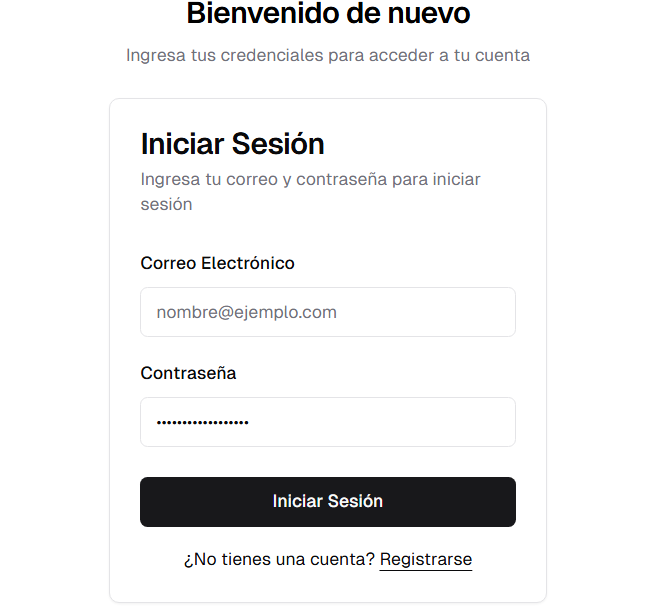
\includegraphics[width=0.6\textwidth]{images/loguin.PNG} % Imagen del ejemplo
			\end{center}
			\medskip
		}
		
	\end{userstory}
	
	\begin{userstory}[hu:03]
		\storyname{Cerrar sesión del sistema}
		\storyuser{Usuario autenticado}
		\storyiter{1} % Iteración estimada
		\storypriority{Media} % Basado en RF3
		\storyrisk{Bajo}
		\storypoints{0.5 semanas} % Estimación basada en ejemplo
		\storyprogrammer{Daniel Rojas Grass}
		\storydescription{
			Como usuario autenticado, debe disponer de una opción clara para cerrar su sesión activa, para asegurar la privacidad de su cuenta y finalizar su interacción con el sistema de forma segura. (Corresponde principalmente a RF3)
			
			\textbf{Precondiciones:}
			\begin{itemize}
				\item El usuario tiene una sesión activa (posee un token válido).
				\item El usuario está en la interfaz principal del sistema.
			\end{itemize}
			
			\textbf{Flujo de acción:}
			\begin{enumerate}
				\item Usuario hace clic en el botón o enlace 'Cerrar Sesión'.
				\item El \textit{frontend} elimina el token de sesión almacenado localmente.
				\item (Recomendado) El \textit{frontend} envía una solicitud al \textit{backend} para invalidar el token en el servidor (si se usa una blacklist de tokens).
				\item El \textit{frontend} redirige al usuario a la página de inicio de sesión o a una página pública principal.
				\item Cualquier intento posterior de acceder a rutas protegidas con el token antiguo debe fallar.
			\end{enumerate}
		}
		\storyobservation{
			El botón de cerrar sesión debe ser fácilmente accesible en la interfaz de usuario autenticado.
		}
		\storyinterface{Botón cerrar sesión en el sitio web:
			\par\medskip % Añade un pequeño espacio vertical
			\begin{center} % Para centrar la imagen
				
\includegraphics[width=0.6\textwidth]{images/cerrar.PNG} % Imagen del ejemplo
			\end{center}
		}
		
	\end{userstory}
	
	% ==========================================
	% Gestión de Conversaciones
	% ==========================================
	
	\begin{userstory}[hu:04]
		\storyname{Iniciar una nueva conversación}
		\storyuser{Usuario autenticado}
		\storyiter{2} % Iteración estimada
		\storypriority{Alta} % Basado en RF5
		\storyrisk{Bajo}
		\storypoints{0.5 semanas} % Estimación basada en ejemplo
		\storyprogrammer{Daniel Rojas Grass}
		\storydescription{
			Como usuario autenticado, debe poder iniciar una nueva conversación de chat en cualquier momento, para realizar consultas sobre temas distintos sin mezclar las interacciones o para empezar una nueva conversación si lo necesita. (Corresponde principalmente a RF5)
			
			\textbf{Precondiciones:}
			\begin{itemize}
				\item El usuario tiene una sesión activa.
				\item El usuario se encuentra en la interfaz principal del chat.
			\end{itemize}
			
			\textbf{Flujo de acción:}
			\begin{enumerate}
				\item Usuario hace clic en la opción "Nueva Conversación" (o icono '+').
				\item El \textit{frontend} limpia el área de visualización del chat actual.
				\item El \textit{frontend} establece un estado interno que indica que la próxima consulta pertenece a una nueva conversación (puede no requerir llamada inmediata al \textit{backend}).
				\item Opcionalmente, el \textit{frontend} puede asignar un ID temporal a la nueva conversación hasta que se envíe el primer mensaje.
				\item La interfaz se muestra lista para recibir la primera consulta de la nueva conversación.
			\end{enumerate}
		}
		\storyobservation{
			La acción debe ser visualmente clara y distinguible de seleccionar una conversación existente. El estado de "nueva conversación" debe manejarse correctamente hasta el primer envío.
		}
		\storyinterface{Botón nueva conversación en el sitio web:
			\par\medskip % Añade un pequeño espacio vertical
			\begin{center} % Para centrar la imagen
				
\includegraphics[width=0.6\textwidth]{images/newConversation.PNG} % Imagen del ejemplo
			\end{center}
			\medskip
		}
		
	\end{userstory}
	
	\begin{userstory}[hu:05]
		\storyname{Ver historial de conversaciones}
		\storyuser{Usuario autenticado}
		\storyiter{2} % Iteración estimada
		\storypriority{Media} % Basado en RF6
		\storyrisk{Bajo}
		\storypoints{1 semana} % Estimación basada en ejemplo
		\storyprogrammer{Daniel Rojas Grass}
		\storydescription{
			Como usuario autenticado, debe ver una lista organizada de sus conversaciones anteriores (por ejemplo, con un título autogenerado o fecha), para poder identificar y acceder fácilmente a interacciones pasadas. (Corresponde principalmente a RF6)
			
			\textbf{Precondiciones:}
			\begin{itemize}
				\item El usuario tiene una sesión activa.
				\item El \textit{backend} y la base de datos que almacena el historial están operativos.
			\end{itemize}
			
			\textbf{Flujo de acción:}
			\begin{enumerate}
				\item El \textit{frontend} (al cargar la interfaz principal o al interactuar con un panel de historial) solicita la lista de conversaciones del usuario al \textit{backend}.
				\item El backend consulta la base de datos para obtener los metadatos de las conversaciones asociadas al usuario autenticado (ID, título/fecha, última actualización).
				\item El \textit{backend} retorna la lista de conversaciones al \textit{frontend}.
				\item El \textit{frontend} muestra la lista en un panel lateral o sección designada, permitiendo al usuario ver los identificadores de cada conversación.
			\end{enumerate}
		}
		\storyobservation{
			Considerar paginación si el historial puede ser muy largo. La generación de títulos/identificadores debe ser útil (e.g., basado en la primera consulta). La lista debe actualizarse si se crea o elimina una conversación.
		}
		\storyinterface{Panel/Sección de Historial en el sitio web:
			\par\medskip % Añade un pequeño espacio vertical
			\begin{center} % Para centrar la imagen
				
\includegraphics[width=0.4\textwidth]{images/histo.PNG} % Imagen del ejemplo
			\end{center}
			\medskip
		}
		
	\end{userstory}
	
	\begin{userstory}[hu:06]
		\storyname{Abrir una conversación del historial}
		\storyuser{Usuario autenticado}
		\storyiter{2} % Iteración estimada
		\storypriority{Media} % Basado en RF7
		\storyrisk{Bajo}
		\storypoints{1 semana} % Estimación basada en ejemplo
		\storyprogrammer{Daniel Rojas Grass}
		\storydescription{
			Como usuario autenticado, debe poder seleccionar una conversación específica de su historial listado, para cargar su contenido completo (consultas y respuestas) en la interfaz principal del chat y, opcionalmente, continuarla. (Corresponde principalmente a RF7)
			
			\textbf{Precondiciones:}
			\begin{itemize}
				\item El usuario tiene una sesión activa.
				\item El usuario está viendo la lista de su historial de conversaciones (HU:05).
				\item El \textit{backend} y la base de datos que almacena el historial están operativos.
			\end{itemize}
			
			\textbf{Flujo de acción:}
			\begin{enumerate}
				\item Usuario hace clic en una conversación específica en la lista del historial.
				\item El \textit{frontend} envía una solicitud al \textit{backend} pidiendo el contenido completo de la conversación seleccionada (pasando su ID).
				\item El \textit{backend} recupera todas las consultas y respuestas asociadas a esa conversación para ese usuario.
				\item El \textit{backend} retorna el historial completo de mensajes de esa conversación al \textit{frontend}.
				\item El \textit{backend} limpia el área de chat actual y muestra los mensajes recuperados en el orden correcto.
				\item El \textit{backend} establece la conversación seleccionada como la "conversación activa" actual.
				\item La interfaz permite al usuario añadir nuevas consultas a esta conversación activa.
			\end{enumerate}
		}
		\storyobservation{
			La carga debe ser eficiente, especialmente para conversaciones largas. La interfaz debe indicar claramente cuál conversación del historial está activa.
		}
		\storyinterface{Interacción con lista de historial y chat principal en el sitio web:
			\par\medskip % Añade un pequeño espacio vertical
			\begin{center} % Para centrar la imagen
				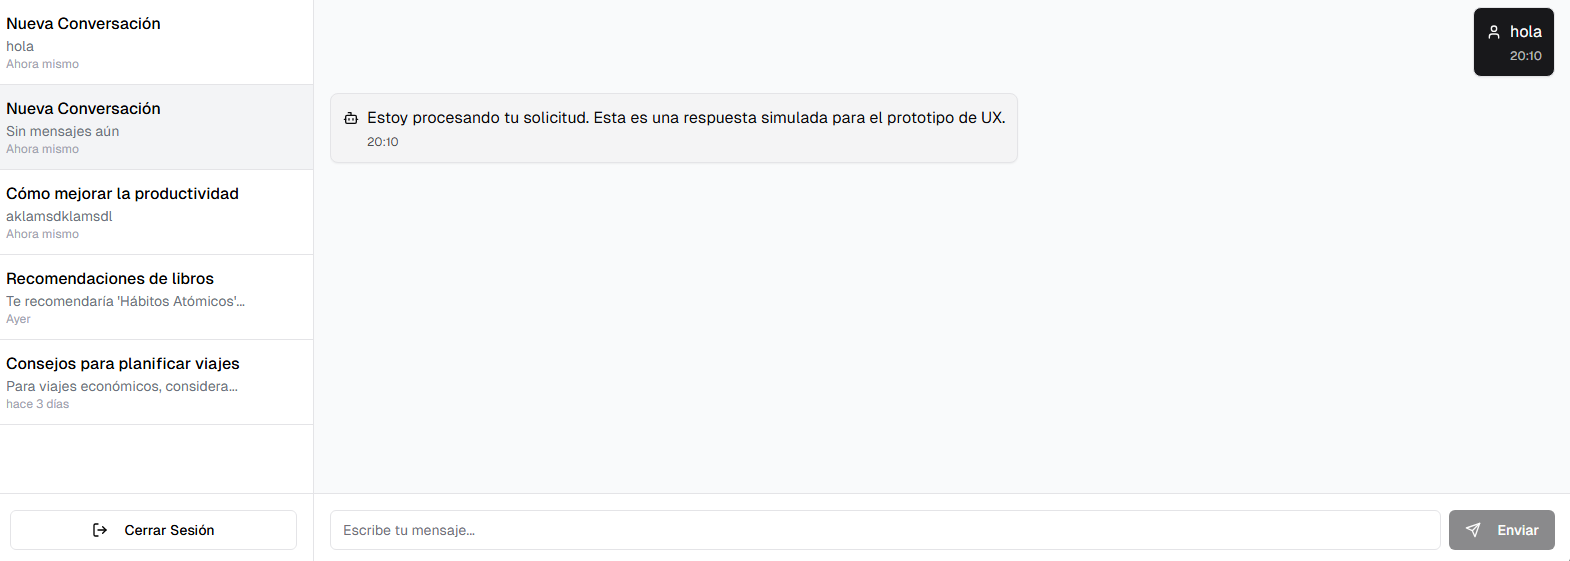
\includegraphics[width=0.6\textwidth]{images/lista.PNG} % Imagen del ejemplo
			\end{center}
			\medskip
		}
		
	\end{userstory}
	
	\begin{userstory}[hu:07]
		\storyname{Eliminar una conversación del historial}
		\storyuser{Usuario autenticado}
		\storyiter{3} % Iteración estimada
		\storypriority{Baja} % Basado en RF8
		\storyrisk{Bajo} % Riesgo de pérdida de datos si no hay confirmación
		\storypoints{1 semana} % Estimación basada en ejemplo
		\storyprogrammer{Daniel Rojas Grass}
		\storydescription{
			Como usuario autenticado, debe tener la opción de eliminar permanentemente una conversación específica de su historial, para mantener su historial limpio y relevante. (Corresponde principalmente a RF8)
			
			\textbf{Precondiciones:}
			\begin{itemize}
				\item El usuario tiene una sesión activa.
				\item El usuario está viendo la lista de su historial o tiene una conversación cargada que desea eliminar.
				\item El \textit{backend} y la base de datos que almacena el historial están operativos.
			\end{itemize}
			
			\textbf{Flujo de acción:}
			\begin{enumerate}
				\item Usuario hace clic en la opción "Eliminar" asociada a una conversación en la lista del historial (o en la conversación activa).
				\item El \textit{frontend} muestra un diálogo de confirmación ("¿Estás seguro de que quieres eliminar esta conversación? Esta acción no se puede deshacer.").
				\item Si el usuario confirma la eliminación:
				\begin{enumerate}
					\item El frontend envía una solicitud al backend DRF para eliminar la conversación (pasando su ID).
					\item El backend verifica que la conversación pertenece al usuario y la elimina de la base de datos.
					\item El backend retorna una respuesta de éxito al frontend.
					\item El frontend elimina la conversación de la lista visible en el historial.
					\item Si la conversación eliminada era la activa, el frontend limpia el área de chat o carga una conversación por defecto/nueva.
				\end{enumerate}
				\item Si el usuario cancela, no se realiza ninguna acción.
			\end{enumerate}
		}
		\storyobservation{
			La confirmación es crucial para prevenir eliminaciones accidentales. La eliminación debe ser lógicamente completa en el backend (borrado permanente).
		}
		\storyinterface{Opción de Eliminar en la lista de Historial o Chat activo:
			\par\medskip % Añade un pequeño espacio vertical
			\begin{center} % Para centrar la imagen
				
\includegraphics[width=0.6\textwidth]{images/eliminarC.PNG} % Imagen del ejemplo (asumiendo que muestra un icono/botón de eliminar)
			\end{center}
			\medskip
		}
		
	\end{userstory}
	
	
	\chapter{Targetas CRC}
		
		\begin{longtable}{|l|l|}
			\caption{Tarjeta CRC: Usuario} \label{tablacrc6} \\
			\hline
			\multicolumn{2}{|c|}{\textbf{Tarjeta CRC}} \\
			\hline
			\textbf{Clase} & \textbf{Usuario} \\
			\hline
			\parbox[t]{0.45\linewidth}{\textbf{Responsabilidades:} \\ 
				Proporcionar datos para registro (email, username, contraseña) \\ 
				Almacenar credenciales de forma segura \\ 
				Mantener información de sesión activa \\ 
				Asociar conversaciones al usuario} 
			& 
			\parbox[t]{0.45\linewidth}{\textbf{Colaboración:} \\ 
				Autenticador \\ 
				BaseDeDatos \\ 
				Conversación} \\
			\hline
		\end{longtable}
		
		\begin{longtable}{|l|l|}
			\caption{Tarjeta CRC: Autenticador} \label{tablacrc7} \\
			\hline
			\multicolumn{2}{|c|}{\textbf{Tarjeta CRC}} \\
			\hline
			\textbf{Clase} & \textbf{Autenticador} \\
			\hline
			\parbox[t]{0.45\linewidth}{\textbf{Responsabilidades:} \\ 
				Validar datos de registro (email único, contraseña fuerte) \\ 
				Autenticar credenciales de inicio de sesión \\ 
				Generar y gestionar tokens de sesión \\ 
				Finalizar sesiones activas} 
			& 
			\parbox[t]{0.45\linewidth}{\textbf{Colaboración:} \\ 
				Usuario \\ 
				BaseDeDatos \\ 
				Backend} \\
			\hline
		\end{longtable}
		
		\begin{longtable}{|l|l|}
			\caption{Tarjeta CRC: Conversación} \label{tablacrc8} \\
			\hline
			\multicolumn{2}{|c|}{\textbf{Tarjeta CRC}} \\
			\hline
			\textbf{Clase} & \textbf{Conversación} \\
			\hline
			\parbox[t]{0.45\linewidth}{\textbf{Responsabilidades:} \\ 
				Iniciar una nueva sesión de chat \\ 
				Almacenar consultas y respuestas \\ 
				Permitir continuación de una conversación existente \\ 
				Eliminar una conversación del historial} 
			& 
			\parbox[t]{0.45\linewidth}{\textbf{Colaboración:} \\ 
				Usuario \\ 
				Historial \\ 
				Backend \\ 
				BaseDeDatos} \\
			\hline
		\end{longtable}
		
		\begin{longtable}{|l|l|}
			\caption{Tarjeta CRC: Historial} \label{tablacrc9} \\
			\hline
			\multicolumn{2}{|c|}{\textbf{Tarjeta CRC}} \\
			\hline
			\textbf{Clase} & \textbf{Historial} \\
			\hline
			\parbox[t]{0.45\linewidth}{\textbf{Responsabilidades:} \\ 
				Listar todas las conversaciones de un usuario \\ 
				Proporcionar metadatos de conversaciones (título, fecha) \\ 
				Permitir selección de una conversación específica} 
			& 
			\parbox[t]{0.45\linewidth}{\textbf{Colaboración:} \\ 
				Usuario \\ 
				Conversación \\ 
				Backend \\ 
				BaseDeDatos} \\
			\hline
		\end{longtable}
		
		\begin{longtable}{|l|l|}
			\caption{Tarjeta CRC: Chat} \label{tablacrc10} \\
			\hline
			\multicolumn{2}{|c|}{\textbf{Tarjeta CRC}} \\
			\hline
			\textbf{Clase} & \textbf{Chat} \\
			\hline
			\parbox[t]{0.45\linewidth}{\textbf{Responsabilidades:} \\ 
				Mostrar la interfaz de chat activo \\ 
				Permitir ingreso de consultas en lenguaje natural \\ 
				Visualizar consultas y respuestas (texto e imágenes) \\ 
				Indicar estado de procesamiento} 
			& 
			\parbox[t]{0.45\linewidth}{\textbf{Colaboración:} \\ 
				Conversación \\ 
				Backend \\ 
				MicroservicioMAS} \\
			\hline
		\end{longtable}
		
		\begin{longtable}{|l|l|}
			\caption{Tarjeta CRC: Backend} \label{tablacrc11} \\
			\hline
			\multicolumn{2}{|c|}{\textbf{Tarjeta CRC}} \\
			\hline
			\textbf{Clase} & \textbf{Backend} \\
			\hline
			\parbox[t]{0.45\linewidth}{\textbf{Responsabilidades:} \\ 
				Gestionar endpoints REST para autenticación y chat \\ 
				Coordinar comunicación entre frontend y MicroservicioMAS \\ 
				Almacenar y recuperar datos de conversaciones \\ 
				Proteger rutas con autenticación} 
			& 
			\parbox[t]{0.45\linewidth}{\textbf{Colaboración:} \\ 
				Usuario \\ 
				Autenticador \\ 
				Conversación \\ 
				Historial \\ 
				Chat \\ 
				MicroservicioMAS \\ 
				BaseDeDatos} \\
			\hline
		\end{longtable}
		
		\begin{longtable}{|l|l|}
			\caption{Tarjeta CRC: BaseDeDatos} \label{tablacrc12} \\
			\hline
			\multicolumn{2}{|c|}{\textbf{Tarjeta CRC}} \\
			\hline
			\textbf{Clase} & \textbf{BaseDeDatos} \\
			\hline
			\parbox[t]{0.45\linewidth}{\textbf{Responsabilidades:} \\ 
				Almacenar datos de usuarios (credenciales, sesiones) \\ 
				Persistir conversaciones y su historial \\ 
				Proveer acceso a datos del \textit{Diario de la Marina} (vectorial y CSV)} 
			& 
			\parbox[t]{0.45\linewidth}{\textbf{Colaboración:} \\ 
				Usuario \\ 
				Autenticador \\ 
				Conversación \\ 
				Historial \\ 
				Backend \\ 
				Agente Recuperador (FAISS) \\ 
				Agente PandasAi} \\
			\hline
		\end{longtable}
		
		\begin{longtable}{|l|l|}
			\caption{Tarjeta CRC: MicroservicioMAS} \label{tablacrc13} \\
			\hline
			\multicolumn{2}{|c|}{\textbf{Tarjeta CRC}} \\
			\hline
			\textbf{Clase} & \textbf{MicroservicioMAS} \\
			\hline
			\parbox[t]{0.45\linewidth}{\textbf{Responsabilidades:} \\ 
				Recibir consultas del backend \\ 
				Coordinar agentes internos para procesar consultas \\ 
				Devolver respuestas procesadas (texto e imágenes) al backend} 
			& 
			\parbox[t]{0.45\linewidth}{\textbf{Colaboración:} \\ 
				Backend \\ 
				Agente Moderador \\ 
				Agente Recuperador (FAISS) \\ 
				Agente Contextualizador \\ 
				Agente de Validación \\ 
				Agente PandasAi} \\
			\hline
		\end{longtable}
		
		
		
		
\end{addendum}
